\documentclass[UTF8]{ctexart}
\usepackage{boxedminipage}
\usepackage[paperwidth=210mm,paperheight=297mm,top=25.4mm,bottom=12.7mm,left=12.7mm,right=12.7mm]{geometry}
%\usepackage{setspace}
\usepackage{float}
\usepackage{hyperref}
\usepackage{graphicx}
\usepackage{enumitem}
%==============================
\renewcommand{\figureautorefname}{图}
%\setstretch{1}
\setenumerate[1]{partopsep=0mm,parsep=\parskip,topsep=0mm}
%==============================
\newcommand{\smalltitle}[1]{{\zihao{4}\bfseries{#1}}\\} 
%==============================
\begin{document}
\zihao{5}

\centering
%==============================
\begin{boxedminipage}{184.6mm}
\centering
\smalltitle{开班准备描述}
\begin{boxedminipage}[t]{101.84mm}
\begin{enumerate}
\item 劳保鞋、静电服、静电手套穿戴整齐。不穿戴手套不得触摸零件。
\item 产线清线,非工作物料隔离。
\end{enumerate}
\end{boxedminipage}
\hfill
\begin{boxedminipage}[t]{78.76mm}
\begin{figure}[H]
\parbox[t]{37.38mm}{
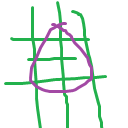
\includegraphics[width=37.38mm]{pic01}
\caption{}\label{afrg}}
\hfill
\parbox[t]{37.38mm}{
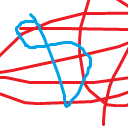
\includegraphics[width=37.38mm]{pic02}
\caption{}}
\end{figure}
\end{boxedminipage}
\end{boxedminipage}
\begin{boxedminipage}{184.6mm}
\centering
\smalltitle{设备开机描述}
\begin{boxedminipage}[t]{101.84mm}
\begin{enumerate}
\item 打开设备总电源,如图一。
\item 按下触摸屏下方的“设备上电”按钮,使其变为绿色,如图二。
\item 人员登录界面,选择“联机模式”,用户名输入“admin”,密码输入“admin”,点击“用户登录”,如图三。
\item 触摸屏点击上方的“目录页面”,随后在右侧选择“自动模式”如图四。
\item 此时触摸屏应当显示“没有报警”,即进入了正常生产模式。如若有报警,请按下触摸屏下方的“回初始位”按钮,设备回到原位后,该按钮应常亮黄色。随后转动“故障复位”旋钮,就能进入自动模式,如图五。
\end{enumerate}
\end{boxedminipage}
\hfill
\begin{boxedminipage}[t]{78.76mm}
图片2
\end{boxedminipage}
\end{boxedminipage}
\autoref{afrg}
\end{document}